\section{函数的连续性与间断点}\label{section:极限.函数的连续性与间断点}

\subsection{函数的连续性}
设变量\(u\)从它的一个初值\(u_1\)变到终值\(u_2\),
终值与初值的差\(u_2 - u_1\)就叫做变量\(u\)的\DefineConcept{增量},
记作\(\increment u\),即\[
	\increment u = u_2 - u_1.
\]

在实数域中,增量\(\increment u\)既可以是正的,也可以是负的.
当\(\increment u > 0\)时,变量\(u\)从初值变到终值时是增大的;
当\(\increment u < 0\)时,变量\(u\)从初值变到终值时是减小的.

应该注意到:
记号\(\increment u\)并不表示某个量\(\Delta\)与变量\(u\)的乘积,
而是一个不可分割的符号.

\begin{definition}\label{definition:极限.函数在一点的连续性}
设函数\(f\colon D\to\mathbb{R}\)在点\(x_0\)的某一邻域内有定义.
如果\[
	\lim_{\increment x\to0} \increment y
	=\lim_{\increment x\to0} [f(x_0 + \increment x)-f(x_0)]
	=0,
\]
或者\[
	\lim_{x \to x_0} f(x) = f(x_0),
\]
或者\[
	(\forall \epsilon > 0)
	(\exists \delta > 0)
	(\forall x \in D)
	[
		0 < \abs{x - x_0} < \delta
		\implies
		\abs{f(x) - f(x_0)} < \epsilon
	],
\]
那么就称“函数\(f(x)\)在点\(x_0\)~\DefineConcept{连续}
(the function \(f(x)\) is continuous at \(x_0\))”,
称“点\(x_0\)是函数\(f(x)\)的\DefineConcept{连续点}(point of continuity)”.

如果\(f(x)\)在点\(x_0\)的某一左邻域内有定义,
极限\(f(x_0^-) = \lim_{x \to x_0^-} f(x)\)存在,且\[
	f(x_0^-) = f(x_0),
\]
则称“函数\(f(x)\)在点\(x_0\)~\DefineConcept{左连续}
(the function \(f(x)\) is left-continuous at \(x_0\))”.

如果\(f(x)\)在点\(x_0\)的某一右邻域内有定义,
极限\(f(x_0^+) = \lim_{x \to x_0^+} f(x)\)存在,且\[
	f(x_0^+) = f(x_0),
\]
则称“函数\(f(x)\)在点\(x_0\)~\DefineConcept{右连续}
(the function \(f(x)\) is right-continuous at \(x_0\))”.
\end{definition}

\begin{figure}[ht]
	\centering
	\def\fn(#1){ln(#1+3)*4-4}
	\begin{tikzpicture}
		\begin{axis}[
			xmin=0,xmax=5,
			ymin=0,ymax=5,
			grid=both,
			xlabel=$x$,
			ylabel=$y$,
			axis equal=true,
			axis lines=middle,
			xtick={1.5,3.5},
			xticklabels={$x_0$,$x_0+\increment x$},
			ytick={\fn(1.5),\fn(3.5)},
			yticklabels={$f(x_0)$,$f(x_0+\increment x)$}
		]
			\addplot[domain=.5:4.5,samples=50,thick,red]{\fn(x)};
		\end{axis}
	\end{tikzpicture}
	\caption{}
\end{figure}

\begin{definition}
如果函数\(f\colon D\to\mathbb{R}\)在\(\forall x \in (a,b)\)处都连续,
那么称“函数\(f\)在开区间\((a,b)\)内连续”,
即\[
	\text{函数\(f\)在\((a,b)\)内连续}
	\defiff
	(\forall x_0\in(a,b))
	[\text{\(f\)在点\(x_0\)连续}].
\]
\end{definition}

\begin{definition}
如果函数\(f\)不仅在\(\forall x \in (a,b)\)处都连续,
还在点\(a\)处右连续,且在\(b\)处左连续,
那么称“函数\(f\)在闭区间\([a,b]\)上连续”.
\end{definition}

类似地可以定义函数\(f(x)\)在半开半闭区间\((a,b]\)或\([a,b)\)内连续的概念.

之前我们在\cref{example:极限.有理整函数在一点的极限} 中研究过有理整函数,
对于任意实数\(x_0\),总有\(\lim_{x \to x_0} f(x) = f(x_0)\),
因此有理整函数在区间\((-\infty,+\infty)\)内是连续的.
而对于有理分式函数\(F(x)=\frac{P(x)}{Q(x)}\),
只要\(Q(x_0)\neq0\),
就有\(\lim_{x \to x_0}F(x)=F(x_0)\),
因此有理分式函数在其定义域内的每一点都是连续的.

由\cref{example:极限.根式函数在某一点的极限} 可知,
函数\(f(x)=\sqrt{x}\)在\((0,+\infty)\)内是连续的.

\begin{example}\label{example:极限.正弦函数在实数域上连续}
证明:函数\(y=\sin x\)在区间\((-\infty,+\infty)\)内是连续的.
\begin{proof}
设\(x\)是区间\((-\infty,+\infty)\)内任意取定的一点.
当\(x\)有增量\(\increment x\)时,对应的函数的增量为\[
	\increment y
	=\sin(x+\increment x)-\sin x.
\]
由和差化积公式有\[
	\sin(x+\increment x)-\sin x
	=2\sin\frac{\increment x}{2}\cos\left(x+\frac{\increment x}{2}\right).
\]
注意到\[
	\abs{\cos\left(x+\frac{\increment x}{2}\right)}\leq1,
\]
就推得\[
	\abs{\increment y}
	=\abs{\sin(x+\increment x)-\sin x}
	\leq2\abs{\sin\frac{\increment x}{2}}.
\]
因为对于任意的角度\(\alpha\),
当\(\alpha\neq0\)时,有\(\abs{\sin\alpha}<\abs{\alpha}\),
所以\[
	0\leq\abs{\increment y}
	=\abs{\sin(x+\increment x)-\sin x}
	<\abs{\increment x}.
\]
因此,当\(\increment x\to0\)时,
由夹逼准则得\(\abs{\increment y}\to0\),
这就证明了\(y=\sin x\)对于任一\(x\in(-\infty,+\infty)\)是连续的.
\end{proof}
\end{example}
类似地可以证明,函数\(y=\cos x\)在区间\((-\infty,+\infty)\)内是连续的.

\begin{definition}\label{definition:函数族.连续函数族}
由区间\(I\)上全部的连续函数组成的集合,称作\DefineConcept{连续函数族},记作\(C(I)\),即\[
	C(I)
	\defeq
	\Set*{
		f\in\mathbb{R}^I
		\given
		(\forall x \in I)
		[\text{\(f\)在点\(x\)处连续}]
	}.
\]
\end{definition}

\begin{example}
证明:若\(f(x)\)在\((-\infty,+\infty)\)内连续,且\(\lim_{x \to \infty}f(x)\)存在,则\(f(x)\)必在\((-\infty,+\infty)\)内有界.
\begin{proof}
因为\(\lim_{x \to \infty} f(x)\)存在,
那么由函数极限的局部有界性定理可知,\[
	(\exists M>0)
	(\exists X>0)
	[
		\abs{x} > X \implies \abs{f(x)} \leq M
	],
\]
也就是说\(f(x)\)在区间\((-\infty,-X)\cup(X,+\infty)\)上有界.

又因为\(f(x)\)在\((-\infty,+\infty)\)内连续,
所以\(f(x)\)在\([-X,X]\)上连续,
进而\(f(x)\)在\([-X,X]\)上有界.

综上所述,\(f(x)\)在\((-\infty,+\infty)\)上有界.
\end{proof}
\end{example}

\begin{example}
设\(f \in C(\mathbb{R})\),
且\((\forall x,y\in\mathbb{R})[f(x+y) = f(x) + f(y)]\).
证明:\[
	(\forall x\in\mathbb{R})[f(x) = f(1) x].
\]
\begin{proof}
\def\f#1#2{f\left(\frac{#1}{#2}\right)}
令\(x=y=0\),得\(f(0+0) = f(0) + f(0)\),移项,得\(f(0) = 0\).

当\(x = m/n \in \mathbb{Q}\)时.
因为\[
	f(1) = \f{1}{n} + \f{n-1}{n}
	= 2 \f{1}{n} + \f{n-2}{n}
	= \dotsb
	= n \f{1}{n},
\]
所以\(f(1/n) = f(1) / n\),进而\[
	\begin{split}
	\f{m}{n}
	&= \f{1}{n} + \f{m-1}{n}
	= 2 \f{1}{n} + \f{m-2}{n} \\
	&= \dotsb
	= m \f{1}{n} = \frac{m}{n} f(1).
	\end{split}
\]

当\(x \in \mathbb{Q}^C\)时.
用有理数列逼近无理数证明题设成立.
\end{proof}
\end{example}

%\subsection{连续曲线}
%\begin{definition}
%设平面曲线\(L\)的参数方程为\[
%	\left\{ \begin{array}{l}
%		x = \phi(t) \\
%		y = \psi(t)
%	\end{array} \right.,
%	\quad
%	t \in [\alpha,\beta].
%\]
%如果\(\phi(t)\)、\(\psi(t)\)在\([\alpha,\beta]\)上连续,
%则称曲线\(L\)为\DefineConcept{连续曲线}.
%点\(\opair{\phi(\alpha),\psi(\alpha)}\)称为曲线的\DefineConcept{起点},
%点\(\opair{\phi(\beta),\psi(\beta)}\)称为曲线的\DefineConcept{终点}.
%
%如果存在\(t_1\)、\(t_2\)满足\(\alpha \leq t_1 < t_2 \leq \beta\)
%且\((t_1-\alpha)^2+(t_2-\beta)^2 \neq 0\),使得对应的两点重合,
%即\(\opair{\phi(t_1),\psi(t_1)}=\opair{\phi(t_2),\psi(t_2)}\)成立,
%则称该点为曲线\(L\)的\DefineConcept{重点}.
%
%无重点的连续曲线称为\DefineConcept{若尔当曲线}或\DefineConcept{简单曲线}.
%
%仅起点和终点重合
%(即\(\opair{\phi(\alpha),\psi(\alpha)}
%=\opair{\phi(\beta),\psi(\beta)}\))
%的简单曲线称作\DefineConcept{若尔当闭曲线}或者\DefineConcept{简单闭曲线}.
%\end{definition}

\subsection{函数的间断点}
设函数\(f(x)\)在点\(x_0\)的某去心邻域内有定义.
在此前提下,如果函数\(f(x)\)有下列三种情形之一:
\begin{enumerate}
	\item 在\(x=x_0\)没有定义;
	\item 虽在\(x=x_0\)有定义,
	但\(\lim_{x \to x_0} f(x)\)不存在;
	\item 虽在\(x=x_0\)有定义,
	且\(\lim_{x \to x_0} f(x)\)存在,
	但\(\lim_{x \to x_0} f(x) \neq f(x_0)\),
\end{enumerate}
则称“函数\(f(x)\)在点\(x_0\)不连续”,
称“点\(x_0\)是函数\(f(x)\)的\DefineConcept{不连续点}或\DefineConcept{间断点}(discontinuity)”.

\begin{figure}[ht]
	\centering
	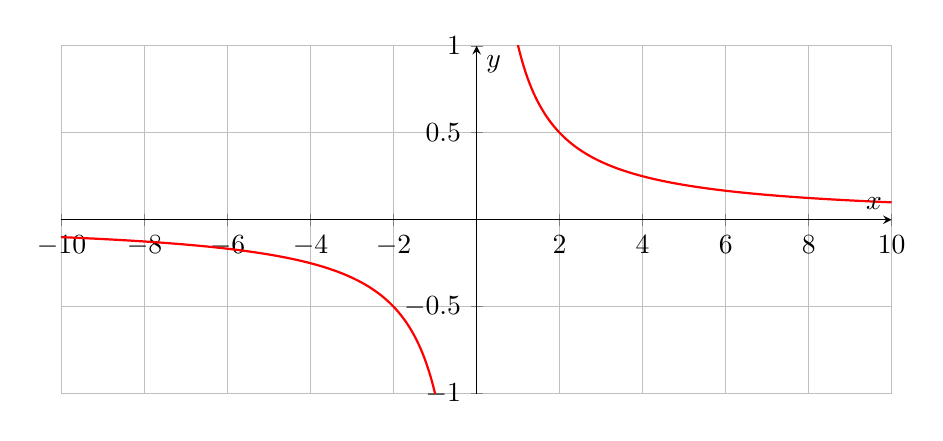
\begin{tikzpicture}
		\begin{axis}[
			xmin=-10,xmax=10,
			ymin=-1,ymax=1,
			grid=both,
			width=\textwidth,
			height=6cm,
			xlabel=$x$,
			ylabel=$y$,
			axis lines=middle,
		]
			\begin{scope}[samples=200,smooth,thick,red]
				\addplot[domain=-10:-.1]{1/x};
				\addplot[domain=+.1:+10]{1/x};
			\end{scope}
		\end{axis}
	\end{tikzpicture}
	\caption{}
	\label{figure:极限.无穷间断点}
\end{figure}

\begin{figure}[ht]
	\centering
	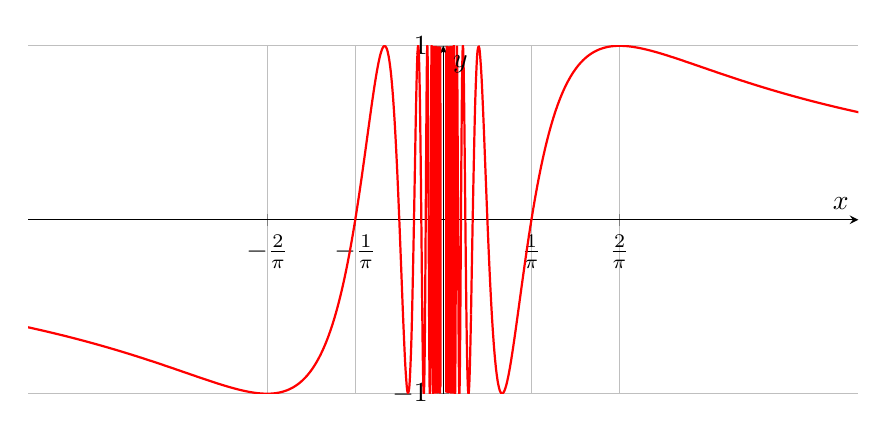
\begin{tikzpicture}
		\begin{axis}[
			xmin=-1.5,xmax=1.5,
			ymin=-1,ymax=1,
			grid=both,
			width=\textwidth,
			height=6cm,
			xlabel=$x$,
			ylabel=$y$,
			axis lines=middle,
			ytick={-1,1},
			xtick={-2/pi,-1/pi,1/pi,2/pi},
			xticklabels={$-\frac{2}{\pi}$,$-\frac{1}{\pi}$,$\frac{1}{\pi}$,$\frac{2}{\pi}$},
		]
			\begin{scope}[samples=200,smooth,thick,red]
				\addplot[domain=-5/pi:-.1]{sin(deg(1/x))};
				\addplot[domain=-.05:-.1]{sin(deg(1/x))};
				\addplot[domain=-.05:-.01]{sin(deg(1/x))};
				\addplot[domain=.05:.1]{sin(deg(1/x))};
				\addplot[domain=.05:.01]{sin(deg(1/x))};
				\addplot[domain=+.1:+5/pi]{sin(deg(1/x))};
			\end{scope}
		\end{axis}
	\end{tikzpicture}
	\caption{}
	\label{figure:极限.振荡间断点}
\end{figure}

如果\(\lim_{x \to x_0}f(x) = \infty\),
则称点\(x_0\)为函数的\DefineConcept{无穷间断点}.
如\cref{figure:极限.无穷间断点},
点\(x=0\)是函数\(y=\frac{1}{x}\)的无穷间断点.

如果\(f(x)\)在点\(x_0\)的某一邻域是有界的,
但其左、右极限均不存在,则称点\(x_0\)为函数的\DefineConcept{振荡间断点}.
如\cref{figure:极限.振荡间断点},
点\(x=0\)是函数\(y=\sin\frac{1}{x}\)的振荡间断点.

如果\(\lim_{x \to x_0}f(x) = A\),
但是\(f(x)\)在点\(x_0\)没有定义,或者\(f(x_0) \neq A\),
则称点\(x_0\)为函数的\DefineConcept{可去间断点}(removable discontinuity).
如\cref{figure:极限.函数[y=sin(x)/x]的图像},
点\(x=0\)是函数\(y=\frac{\sin x}{x}\)的可去间断点.

如果\(f(x)\)在点\(x_0\)的左、右极限存在但不相等,
即\(\lim_{x \to x_0^-}f(x) \neq \lim_{x \to x_0^+}f(x)\),
则称点\(x_0\)为函数的\DefineConcept{跳跃间断点}(jump discontinuity).

如果\(x_0\)是函数\(f(x)\)的间断点,
但左极限\(f(x_0^-)\)及右极限\(f(x_0^+)\)都存在,
那么\(x_0\)称为函数\(f(x)\)的\DefineConcept{第一类间断点}(discontinuity of the first kind).
不是第一类间断点的间断点,称为\DefineConcept{第二类间断点}(discontinuity of the second kind).

显然,可去间断点、跳跃间断点是第一类间断点,
无穷间断点、振荡间断点是第二类间断点.

\begin{example}\label{example:极限.狄利克雷函数在实数域上处处不连续}
证明:狄利克雷函数\[
D(x) = \left\{ \begin{array}{ll}
1, & x \in \mathbb{Q}, \\
0, & x \in \mathbb{R} - \mathbb{Q}.
\end{array} \right.
\]在\(\mathbb{R}\)上处处不连续.
\begin{proof}
\(\forall x_0 \in \mathbb{R}\),一定存在全由有理数组成的数列\(\{s_n\}\)和全由无理数组成的数列\(\{t_n\}\)趋于点\(x_0\),这样就有\[
\lim_{n\to\infty} D(s_n) = 1,
\qquad
\lim_{n\to\infty} D(t_n) = 0.
\]
根据\hyperref[theorem:极限.海涅定理]{海涅定理}可知,\(\lim_{x \to x_0} D(x)\)不存在.
\end{proof}
\end{example}

\begin{example}
证明:函数\(f(x) = x D(x)\)除在点\(x = 0\)处连续之外,在\(\mathbb{R}\)上其余各点均不连续.
\begin{proof}
先证\(f\)在点\(x = 0\)处连续.此时\(f(0) = 0\).
\(\forall \epsilon > 0\),取\(\delta = \epsilon\),当\(\abs{x - 0} = \abs{x} < \delta\)时,有\[
\abs{f(x) - f(0)}
= \abs{ x D(x) }
\leq \abs{x} < \delta = \epsilon,
\]故\(f\)在点\(x = 0\)处连续.

当\(x \neq 0\)时,有\(D(x) = \frac{f(x)}{x}\).用反证法.假设\(f\)在点\(x_0 \neq 0\)处连续,那么\[
\lim_{x \to x_0} D(x) = \lim_{x \to x_0} \frac{f(x)}{x}
= \frac{ \lim_{x \to x_0} f(x) }{x_0}
= \frac{f(x_0)}{x_0} = D(x_0),
\]也就是说狄利克雷函数\(D(x)\)在点\(x_0\)处连续,矛盾!故\(f\)在点\(x \neq 0\)处不连续.
\end{proof}
\end{example}

上述两个例子说明,存在处处不连续的函数,也存在只有一个连续点的函数.

\begin{example}
证明:\DefineConcept{黎曼函数}\[
	R(x) = \left\{ \begin{array}{cl}
		\frac{1}{n},
			& x=\frac{m}{n}\in\mathbb{Q}-\{0\}
				\land n\in\mathbb{N}^+
				\land \gcd{m,n}=1, \\
		0, & x\in(\mathbb{R}-\mathbb{Q})\cup\{0\}
	\end{array} \right.
\]在有理数点处不连续,在无理数点处连续.
%TODO
\end{example}

\begin{example}
已知函数\(f(x) = \frac{x-x^3}{\sin \pi x}\),求该函数的可去间断点的个数.
\begin{solution}
当\(\sin \pi x = 0\)或\(x \in \mathbb{Z}\)时,函数\(f\)无定义;也就是说,点\(x\in\mathbb{Z}\)都是\(f\)的间断点.
要使点\(x\)成为函数\(f\)的可去间断点,必有\(x-x^3=0\),即\(x=0,\pm1\).
\def\l#1{\lim_{x\to#1}}%
又因为\[
\l{0} \frac{x-x^3}{\sin \pi x}
= \l{0} \frac{x(1-x^2)}{\pi x}
= \frac{1}{\pi},
\]\[
\l{1} \frac{x-x^3}{\sin \pi x}
= \l{1} \frac{1-3x^2}{\pi \cos \pi x}
= \frac{2}{\pi},
\]\[
\l{-1} \frac{x-x^3}{\sin \pi x}
= \l{-1} \frac{1-3x^2}{\pi \cos \pi x}
= \frac{2}{\pi},
\]综上,函数\(f\)共有3个可去间断点.
\end{solution}
\end{example}

\begin{example}
设函数\(f(x) = \frac{x^2-x}{x^2-1}\sqrt{1+\frac{1}{x^2}}\).
试计算\(f(x)\)的间断点种类及其个数.
\begin{solution}
因为\[
f(x) = \frac{x(x-1)}{(x-1)(x+1)} \frac{\sqrt{x^2+1}}{\abs{x}},
\]所以\(f(x)\)的间断点为\(x=0,\pm1\).

又因为\begin{align*}
&\lim_{x\to1} f(x)
= \lim_{x\to1} \frac{\sqrt{x^2+1}}{x+1}
= \frac{\sqrt{2}}{2}, \\
&\lim_{x\to0^+} f(x)
= \lim_{x\to0^+} \frac{\sqrt{x^2+1}}{x+1}
= 1, \\
&\lim_{x\to0^-} f(x)
= \lim_{x\to0^-} -\frac{\sqrt{x^2+1}}{x+1}
= -1, \\
&\lim_{x\to-1} f(x)
= \lim_{x\to-1} \frac{\sqrt{x^2+1}}{x+1}
= \infty,
\end{align*}
所以点\(x=1\)是可去间断点,点\(x=0\)是跳跃间断点,点\(x=-1\)是无穷间断点.
那么可去间断点、跳跃间断点和无穷间断点的个数均为1个.
\end{solution}
\end{example}

\subsection{狄利克雷函数}
我们在\cref{example:极限.狄利克雷函数在实数域上处处不连续} 中已经看到,狄利克雷函数\[
D(x) = \left\{ \begin{array}{ll}
1, & x \in \mathbb{Q}, \\
0, & x \in \mathbb{R} - \mathbb{Q}.
\end{array} \right.
\]在实数域\(\mathbb{R}\)上处处不连续.

下面介绍狄利克雷函数的另一种构造方法:
\begin{example}
证明:\[
D(x) = \lim_{n\to+\infty} \lim_{k\to+\infty} \cos^{2k}(n! \pi x).
\]
\begin{proof}
设\(a_n = \lim_{k\to+\infty} \cos^{2k}(n! \pi x)\).

当\(x \in \mathbb{Q}\)时,\(x\)必可表为两个既约整数的比,不妨设\(q/p\),那么\[
a_p = \lim_{k\to+\infty} \cos^{2k}\left(p! \pi \frac{q}{p}\right)
= \lim_{k\to+\infty} \cos^{2k}[(p-1)! \pi q] = 1.
\]故\[
D(x) = \lim_{n\to+\infty} a_n = 1.
\]

当\(x \in \mathbb{R}-\mathbb{Q}\)时,\(n! x \in \mathbb{R}-\mathbb{Q}\),因此\[
\cos(n! \pi x) \in (-1,1),
\]从而\[
a_n = \lim_{k\to+\infty} \cos^{2k}(n! \pi x) = 0,
\]故\[
D(x) = \lim_{n\to+\infty} a_n = 0.
\]

综上所述,\(D(x) = \lim_{n\to+\infty} \lim_{k\to+\infty} \cos^{2k}(n! \pi x)\).
\end{proof}
\end{example}

\subsection{半连续性}
\begin{definition}
设\(f\colon D\to\mathbb{R}\).
规定:\[
	\begin{split}
		\text{\(f\)在点\(x_0\) \DefineConcept{上半连续}}
		\defiff
			&\text{\(f\)在\(D\)内有上界} \\
			&\land
			(\forall\epsilon>0)
			(\exists\delta>0)
			(\forall x \in D)
			[
				\abs{x-x_0}<\delta
				\implies
				f(x)<f(x_0)+\epsilon
			]; \\
		\text{\(f\)在点\(x_0\) \DefineConcept{下半连续}}
		\defiff
			&\text{\(f\)在\(D\)内有下界} \\
			&\land
			(\forall\epsilon>0)
			(\exists\delta>0)
			(\forall x \in D)
			[
				\abs{x-x_0}<\delta
				\implies
				f(x)>f(x_0)-\epsilon
			].
	\end{split}
\]
%@see: https://healy.econ.ohio-state.edu/kcb/Ec181/Lecture13.pdf
\end{definition}
